\documentclass[9pts]{article}
\usepackage[utf8]{inputenc}
\usepackage[a4paper,top=2.5cm, bottom=3.5cm, left=1.5cm, right=1.5cm]{geometry}

\usepackage{listings}
\usepackage{color}
\usepackage{graphicx}
\usepackage{caption}
\usepackage{fancyhdr}
\usepackage{appendix}
\usepackage{inconsolata}
% \usepackage{fontspec}
\usepackage{titling}
\usepackage{hyperref}

\renewcommand{\ttdefault}{cmtt}

%% \usepackage[a4paper,margin=2.5cm,bottom=2cm,headheight=1cm]{geometry}
\pagestyle{fancy}
\fancyhead[L]{\hspace*{-2.5mm} 
\includegraphics[scale=0.1]{./faculte_sciences_sorbonne_logo.png}}
\fancyhead[R]{\includegraphics[scale=0.27]{./master-SPI-logo.jpg} \vspace*{0.1mm}}
\fancyfoot[C]{}
\renewcommand{\headrulewidth}{0pt}

\definecolor{mygreen}{rgb}{0,0.6,0}
\definecolor{mygray}{rgb}{0.5,0.5,0.5}
\definecolor{mymauve}{rgb}{0.58,0,0.82}

\definecolor{bluekeywords}{rgb}{0,0,1}
\definecolor{greencomments}{rgb}{0,0.5,0}
\definecolor{redstrings}{rgb}{0.64,0.08,0.08}
\definecolor{xmlcomments}{rgb}{0.5,0.5,0.5}
\definecolor{types}{rgb}{0.17,0.57,0.68}
\lstdefinestyle{mystyle}{
  captionpos=b,
  %numbers=left,
  %numberstyle=\tiny,
  frame=lines,
  showspaces=false,
  showtabs=false,
  breaklines=true,
  showstringspaces=false,
  breakatwhitespace=true,
  escapeinside={(*@}{@*)},
  commentstyle=\color{greencomments},
  morekeywords={partial, var, value, get, set},
  keywordstyle=\color{bluekeywords},
  stringstyle=\color{redstrings},
  basicstyle=\ttfamily\small,
}
\lstset{style=mystyle}

\setlength{\droptitle}{1em}
\title{[4AI02] Projet de C++ Avancé: Application RATP}
\date{9 Avril 2019}

\begin{document}
\makeatletter

\let\ps@plain=\ps@fancy

\makeatother
\maketitle

Trois séances de 4H sont mises à disposition pour réaliser ce projet.
Les étapes à réaliser sont suggérées dans la feuille de route au chapitre \ref{sec::feuille}. Le rythme n'est pas imposé étant donné que la soumission du projet est possible à tout moment lors de la période du projet.
Des programmes de test sont fournis afin d'évaluer le code et d'estimer le niveau d'accomplissement du projet.\\

Notation :
\begin{itemize}
\item Instantiation des classes ($+$3pts $=>$ 3$/$20);
\item Implémentation de read\_stations ($+$3pts $=>$ 6$/$20);
\item Implémentation de read\_connections ($+$3pts $=>$ 9$/$20);
\item Génération du graphe ($+$4pts $=>$ 13$/$20);
\item Estimation du meilleur chemin et affichage ($+$7pts $=>$ 20$/$20);
\item Amélioration ($+$5pts $=>$ 25$/$20);
\item Les critères non respectés de la charte d'écriture (Voir Chapitre \ref{sec::charte}) fera perdre jusqu'a 1 point par critère ($-1$pt).
\item Une mauvaise gestion des exceptions fera perdre 2 points ($-2$pts).\\
\end{itemize}

Les points au dessus de 20 pourront être utilisés comme bonus.\\

Date limite du rendu du code : \textbf{Vendredi 17 mai 2019, 20h00}. Chaque minute de retard fera perdre un point sur la note du projet. Un rendu doit contenir le code nécéssaire pour pouvoir compiler le projet en une seule commande, de même pour l'éxécution. Ces commandes peuvent être définies par exemple dans un fichier \emph{lisez-moi}. \\

La soumission du projet se fera sur l'espace Moodle dédié. La soumission multiple est possible, la dernière soumission écrasant les précédentes. Il est fortement encouragé de soumettre à chaque étape de résolution du projet.

\pagebreak
\renewcommand{\headrulewidth}{0.5pt}
\fancyhead[LO,RE]{
\includegraphics[scale=0.06]{./faculte_sciences_sorbonne_logo.png}}
\fancyhead[RO,LE]{\includegraphics[scale=0.17]{./master-SPI-logo.jpg}}
\fancyfoot[C]{\thepage}

\section{Introduction}
Vous êtes membre d'une start-up qui veut se lancer sur le marché de la vente de données de trafic.
L'équipe de développement vous demande d'implémenter un algorithme capable de planifier des temps de parcours au moyen d'une heuristique fixe, ou dynamique.
Une base de données réaliste et fiable pour le tester est requise. Celle-ci permettera d'établir la validité de l'algorithme, et du cadre dans lequel va naître le projet.
L'algorithme de Dijkstra et la base de données de la RATP sont des choix logiques car robustes.
Après concertation, un contrat de programmation est écrit, afin de juger des fonctionnalités minimales ne ralentissant pas l'évolutivité de la solution.
La tâche est de réaliser un programme respectant la structure imposée. Une recherche sera nécéssaire afin de maîtriser l'algorithme de Dijkstra, afin de pouvoir l'implémenter.

\subsection{Une résolution du problème du plus court chemin}
Le but de ce projet est de faire une application qui établit le trajet le plus court entre deux stations du réseau de métro parisien.

\begin{figure}[h]
   \centering
   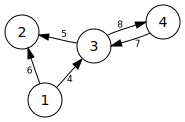
\includegraphics[width=9cm,keepaspectratio]{directed_graph.pdf}
   \caption{\label{directed_graph} Exemple de graphe orienté}
\end{figure}

En théorie des graphes, un graphe orienté est un ensemble de points (ici, des entrées de stations de métro) connectés par des liens orientés (ici, les connexions entre les stations, en secondes). Dans le cadre de ce projet, chaque lien représente une possibilité de relier deux points, dans un sens précis, et avec un coût déterminé. C'est une connection possible entre ces points.

Le problème du plus court chemin, dans ce système, est d'évaluer le coût minimal pour aller d'un point A à un point B. L'algorithme de Dijkstra est une méthode de calcul afin de résoudre ce problème.\\

\label{sec::path_vector_example}
Par exemple, dans le graphe de la Figure 1, le chemin le plus court entre le noeud B et le noeud G passe par les noeuds A et C, pour un coût cumulé de 85$+$217$+$186$=$488. Ce chemin peut être exprimé comme une liste de noeuds et le coût cumulé du chemin, ici, {\color{blue} $best\_path = [\{B, 0\}, \{A, 85\}, \{C, 302\}, \{D, 488\}]$};

Cet algorithme peut s'appliquer sur des graphes orientés, modèle auquel plusieurs réseaux de transports sont disponibles (RATP, SNCF, routes, etc), et est également une porte d'entrée pour le domaine de la théorie des graphes et de la théorie de la décision.\\

\subsection{Méthode de développement, et outils de la \emph{STL}}

Un programme informatique est une suite d'instructions mathématiques. A ce titre il existe deux difficultés lorsque l'on veut construire un programme informatique pour répondre à un problème :
\begin{enumerate}
\item Quel jeu d'instructions choisir pour répondre au problème algorithmique?\\
La solution ici a été trouvée par l'informaticien Edsger Dijkstra, répondant au problème du plus court chemin énoncée ci-dessus.

\item Comment structurer, implémenter mon problème algorithmique, qui requiert ici la construction de centaines de milliers d'instructions machine, avec la méthodologie nécéssaire pour que n'importe quel humain puisse maintenir ce code et y ajouter des fonctionnalités?\\
Cette question est en partie résolue par l'outil C++. C'est une méthodologie, permettant de générer une grande compléxité dans le jeu d'instructions (comme beaucoup d'outils informatiques), mais également d'utiliser une interface compréhensible, qui vous est donnée ici, et va permettre l'ajout de fonctionnalités de manière concise et ergonomique, en détachant les différentes fonctionnalités, permettant de fournir au final une solution élégante et ré-utilisable.
\end{enumerate}


Afin de résoudre ce problème, des fichiers contenant les points d'un graphe, et contenant des connexions, sont mis à votre disposition. La lecture de ces fichiers devra être réalisée avec des conteneurs spécifiques imposés. Puis, un calcul du chemin le plus court devra être réalisé.\\

Afin de travailler les connaissances vues en cours, nous allons utiliser la \emph{Standard Template Library}, une bibliothèque C++ parmi tant d'autres, mais qui a l'avantage d'être très puissante dans plusieurs modalités, notamment pour les conteneurs que celle-ci propose. Ceux-ci représentent des tableaux associatifs, généralisation des tableaux où les indices ne sont pas forcément des entiers.\\

\begin{figure}[h]
   \centering
   \includegraphics[width=18cm,keepaspectratio]{ratp_graph.pdf}
   \caption{\label{directed_graph} Graphe orienté généré à partir des fichiers \texttt{c.csv} et \texttt{s.csv}, avec les données GPS des stations.}
\end{figure}

Une table de hachage est une structure de données efficace pour représenter un tableau associatif, avec une réprésentation mémoire compacte, via le hachage des données qui, dans ce cas, associe une information (la station) à une clé (l'identifiant de station). Les éléments à insérer dans le conteneur ne sont pas forcément triés. Ce sont les raisons pour lesquelles nous utiliseront le conteneur \texttt{std::unordered\_map}, ressemblant (d'un point de vue utilisateur) au conteneur \texttt{std::map} vu en cours, qui implémente lui un arbre binaire de recherche pour garantir l'ordre des données.

Ces conteneurs vont garder les données du graphe fourni via des fichiers qu'il faudra lire et dont les données doivent être extraites.
Dans ce cas précis, l'utilisation de la bibliothèque standard est fortement conseillé, via la classe \texttt{std::ifstream}, prenant en argument le nom du fichier à lire. Une des différentes méthodes pour lire une ligne est d'utiliser la fonction membre \texttt{getline}.\\

Une auto-évaluation vous est proposée au chapitre \ref{sec::autoeval}, afin de construire progressivement les fonctions nécéssaires à l'accomplissement du projet, et d'ajuster le temps nécéssaire pour le terminer.

\section{Charte d'écriture}
\label{sec::charte}
Ce projet vous impose une charte d'écriture afin de pouvoir maintenir le code et faciliter sa transmission. Cette charte est énoncée dans un ordre quelconque:\\

\begin{itemize}
\item \textbf{Utilisation des drapeaux de compilation -Wall -Wextra -Werror -pedantic -pedantic-errors -O3 de g++} afin de garantir le respect de l'implémentation dans les normes C++, et d'optimiser la compilation;
\item \textbf{Utilisation des fonctionnalités du C++ 11 maximum} afin d'utiliser les ressources du cours. Le drapeau de compilation \emph{std=c++11} pourra être utilisé; %https://msdn.microsoft.com/fr-fr/library/hh567368.aspx
\item \textbf{Minimisation de l'utilisation des outils d'allocation dynamique} : \emph{new}, \emph{new[]}, \emph{delete} et \emph{delete[]}, afin d'optimiser la sécurité, la lisibilité, et de tirer parti du concept \emph{RAII} : l'acquisition d'une ressource est une initialisation. Ce projet est faisable sans allocation dynamique, cela sera apprécié et simplifiera votre projet;
\item \textbf{Mémoire dynamique via les conteneurs de la \emph{STL}};
\item \textbf{Indentation parfaite du code source du programme} afin de garantir la lisibilité et de prévenir les erreurs d'implémentation;
\item \textbf{Minimisation de duplication du code source du programme} afin d'éviter le dangereux copier-coller et les graves problèmes de maintenance induits par ce comportement;
\item \textbf{Utilisation de la convention \emph{snake\_case}}, avec des noms de fonctions en \emph{verbe\_complément}, de variables en \emph{complément\_nom}, afin de garantir la lisibilité du code;
\item \textbf{Tout type créé commence par une majuscule}, par convention;
\item \textbf{Les constantes déclarées via \emph{define} sont écrites intégralement en majuscules}; on parlera ici de \emph{SCREAMING\_SNAKE\_CASE};
\item \textbf{Membres de classes appelés via \emph{this}} afin de répèrer facilement l'utilisation et la modification d'outils interne;
\item \textbf{Variables d'entrées précédées d'un underscore \emph{\_}}, pour faciliter la différenciation avec les autres types de variables;
% \item \textbf{Variables locales neutres}; % kézako
\item \textbf{Utilisation du mot clef \emph{const} lorsque l'entrée ne doit pas être modifiée}, afin de garantir ses droits d'accès en lecture/écriture;
\item \textbf{Utilisation systématique de référence ou de pointeur lors du passage d'un objet}, les objets seront passés par copie;
% \item \textbf{Respect du typage lors des comparaisons au moyen de \emph{static\_cast$<$Type$>$(var)} si nécessaire}.
% \item \textbf{Utilisation du drapeau de compilation -fsyntax-only lors de la compilation de fichiers entête}, afin de forcer le compilateur à recompiler les fichiers entête à chaque modification. La compilation de fichiers entête n'est pas indispensable au bon déroulement du projet.
\end{itemize}

\pagebreak

\section{Objectifs}

Un des buts de ce projet est de permettre l'assemblage de code de plus en plus complet, avec un écosystème compréhensible alors qu'il grossit. La méthodologie va montrer cette difficulté, et
c'est pourquoi les objets englobent ces fonctionnalités. \\

Le point le plus important dans le cadre de ce projet est de comprendre l'interface, la structure imposée. Le travail demandé, qui est d'implémenter les fonctionnalités clés, ne sera pas possible sans la compréhension de cette structure. Il est aussi judicieux de se renseigner sur les outils possibles et nécéssaires pour réussir le projet.\\

Les classes doivent hériter d'une classe mère virtuelle pure sans implémentation. Ce principe permet de rajouter des fonctionnalités à une classe sans l'altérer et en garantissant son appel via un pointeur.
Si la classe respecte le contrat, elle garantit d'avoir implémenté les fonctionnalités nécéssaires à la validité du programme. Cela n'empeche pas de pouvoir améliorer et ajouter diverses fonctionnalités supplémentaires, notamment celle proposée en amélioration dans le chapitre \ref{sec::feuille}. \\

\section{Auto-évaluation}
\label{sec::autoeval}
Parmi les fichiers de l'archive du projet se trouve la classe \texttt{Grade} au travers du fichier d'entête \texttt{Grade.hpp} et du fichier objet \texttt{Grade.o}.\\

Ce fichier objet, compilé via le compilateur g++ avec un ordinateur sous Unix, permet une auto-évaluation.

En incluant le fichier binaire à la compilation et à l'entête au programme principal du projet, deux objets statiques sont automatiquement créés. Ceux-ci permettent l'évaluation des différentes parties du projet.
Pour rappel, un objet statique est un objet alloué au lancement du programme et détruit à sa toute fin (par exemple : \texttt{std::cout}, \texttt{std::cin}). Il est non rédéfinissable, pour l'ensemble du code à sa portée.\\

Ces deux objets se nomment ici \texttt{travel::evaluate\_small} et \texttt{travel::evaluate}. Le premier permet d'évaluer le réseau simple, le second évaluant le réseau RATP.\\

Trois méthodes sont disponibles :
\begin{itemize}
  \item \texttt{stations(const travel::Generic\_station\_parser\&)}, qui évalue de manière exhaustive la construction de la table de stations.
  \item \texttt{connections(const travel::Generic\_connection\_parser\&)}, qui évalue de manière exhaustive la construction de la table de connections.
  \item \texttt{dijkstra(travel::Generic\_mapper\&,bool)}, qui évalue dans un premier temps quelques trajets tests, puis propose une exploration exhaustive des trajets via une estimation grossière du temps de calcul.
    \begin{itemize}
      \item Si l'argument booléen est vrai : L'évaluation du projet est faite dans sa version de fin de séances de TP. Le temps de calcul pour le réseau RATP est d'environ 0.3ms/trajet, pour 6 minutes de test.
      \item Si l'argument booléen est faux : L'évaluation du projet est faite dans sa version améliorée, via l'utilisation de noms de stations. Le temps de calcul pour le réseau RATP est cinq fois plus long.
    \end{itemize}
\end{itemize}

Attention : La dernière méthode \texttt{dijkstra(travel::Generic\_mapper\&,bool)} va vérifier la validité des trajets, et ceci dans une certain format. Ce format est d'avoir en liste de noeuds le premier noeud et le dernier noeud dans le trajet, et un coût cumulé associé à chaque noeud, comme dans l'exemple de la section \ref{sec::path_vector_example}.\\

Lorsque une méthode est appelée, elle appelle automatiquement les méthodes précédentes pour garantir le maintien des acquis au fur et à mesure de l'avancement du projet ; Il n'est donc pas nécessaire d'appeler les anciens tests.

De plus, il est à noter que la classe de test est totalement indépendante des classes abstraites et apporte toujours une résolution via les fichiers de références du projet. En définitive, des appels à cette classe seraient appréciés, mais ne sont pas du tout obligatoires dans le cadre du projet.

N'oubliez pas que l'interface vous est imposée, et que vous ne devez pas modifier ces fichiers. La correction sera faite avec seulement l'implémentation de votre classe. Si celle-ci ne se base pas sur l'interface donnée, le code ne sera pas fonctionnel, et vous serez pénalisé.

\pagebreak

\section{Feuille de route}
\label{sec::feuille}
L'équipe de développement de votre start-up vous propose une feuille de route, permettant de représenter les diverses tâches et l'avancement du projet :

\begin{enumerate}
\item Instanciez une classe dérivée : faites un nouveau fichier, une inclusion de la classe parente et créez une classe qui hérite de la classe mère \texttt{Generic\_station\_parser}.\\
Compilez votre fichier de classe. Celui-ci ne doit pas générer d'erreur, même avec les restrictions de compilation imposées dans la charte d'écriture.

\item Créez un fichier avec une fonction principale, et instanciez un objet de votre classe. Le code compile-t-il? Pourquoi?

\item Surchargez la fonction \texttt{Generic\_station\_parser::read\_stations} : Dans la déclaration de la classe, écrivez le prototype de cette fonction \texttt{protected} en ajoutant à la fin le mot clé \texttt{override}. Implémentez cette fonction.

\item Dans votre fonction principale, instanciez votre classe et appelez la méthode \texttt{stations} de la classe \texttt{Grade}. Vous utiliserez l'objet statique mis a disposition dans cette classe, selon la base de données utilisée.\\

\emph{A ce point, vous devriez avoir soumis une version fonctionnelle de votre projet sur Moodle, et ne pas encore avoir eu la deuxième séance de TP.}\\

\item Changez votre classe pour qu'elle hérite de la classe mère \texttt{Generic\_connection\_parser}.\\
Le code compile-t-il, pourquoi?
\item Implémentez la fonction \texttt{read\_connections}.
\item Instanciez votre classe et appelez la méthode \texttt{connections} de la classe \texttt{Grade}.\\

\emph{A ce point, vous devriez avoir soumis une nouvelle version fonctionnelle de votre projet sur Moodle, et ne pas encore avoir eu la troisième séance de TP.}\\

\item Changez votre classe pour qu'elle hérite de la classe mère \texttt{Generic\_mapper}.\\
Le code compile-t-il, pourquoi?
\item Implémentez la fonction \texttt{compute\_travel}, ayant comme arguments d'entrée des nombres correspondant aux identifiants de station. Cette fonction rend un vecteur de \texttt{std::pair}, contenant l'identifiant de la station et le coût associé de la connexion.

\item Implémentez la fonction \texttt{compute\_and\_display\_travel}, permettant d'afficher le chemin calculé par la fonction précédent pour relier les deux stations que vous voulez relier. La notation est dépendante de la clarté de l'affichage, étant donné que le client doit suivre facilement des instructions claires pour se déplacer.
\item Instanciez votre classe et appelez la méthode \texttt{dijkstra} de la classe \texttt{Grade}, avec l'argument booléen à \texttt{false}.\\

\emph{A ce point, vous avez débloqué l'accès aux 20 premiers points de la notation sur le code du projet.}\\

\item Implémentez une surcharge des fonctions qui estiment le trajet minimal pour relier les stations via leurs noms, et non plus leurs identifiants. Il serait convenable d'être résistant aux erreurs (casse, mauvaise orthographe, etc) lors de la saisie des noms par l'utilisateur.

\item Instanciez votre classe et appelez la méthode \texttt{dijkstra} de la classe \texttt{Grade}, avec l'argument booléen à \texttt{true}.
\end{enumerate}

\appendix
\clearpage

\renewcommand{\ttdefault}{zi4}

\section{Interface : Generic\_station\_parser.hpp}
\lstinputlisting[linerange={3-12,17-19,26-32},language=C++]{../v2/Generic_station_parser.hpp}
\section{Interface : Generic\_connection\_parser.hpp}
\lstinputlisting[linerange={3-6,12-19},language=C++]{../v2/Generic_connection_parser.hpp}
\section{Interface : Generic\_mapper.hpp}
\lstinputlisting[linerange={3-13,20-21},language=C++]{../v2/Generic_mapper.hpp}
% \pagebreak
% \section{Pour rappel:}
% \begin{center}
%   \vspace*{\fill}
%   \includegraphics[scale=0.7]{./xkcd.png}
%   \vspace*{\fill}
%   \vspace*{30mm}
% \end{center}
\end{document}
